\documentclass[12pt]{article}
\usepackage{amsmath}
\usepackage{amssymb}
\usepackage[letterpaper,margin=0.85in,centering]{geometry}
\usepackage{fancyhdr}
\usepackage{enumerate}
\usepackage{lastpage}
\usepackage{multicol}
\usepackage{graphicx}

%\reversemarginpar

\pagestyle{fancy}
\cfoot{Page \thepage \ of \pageref{LastPage}}\rfoot{{\bf Total Points: 40}}
\chead{MATH 53}\lhead{Test \# 3}\rhead{Friday, 12\textsuperscript{th} April, 2013}

\newcommand{\points}[1]{\marginpar{\hspace{24pt}[#1]}}
\newcommand{\skipline}{\vspace{12pt}}
%\renewcommand{\headrulewidth}{0in}
\headheight 30pt

\newcommand{\di}{\displaystyle}
\newcommand{\R}{\mathbb{R}}
\newcommand{\aaa}{\mathbf{a}}
\newcommand{\bbb}{\mathbf{b}}
\newcommand{\ccc}{\mathbf{c}}
\newcommand{\dotp}{\boldsymbol{\cdot}}
\newcommand{\pd}[2]{\frac{\partial #1}{\partial #2}}
\newcommand{\rd}[2]{\frac{d #1}{d #2}}
\begin{document}

\author{Instructor: Sean Fitzpatrick}
\thispagestyle{plain}
\begin{center}
\emph{University of California, Berkeley}\\
Department of Mathematics\\
12\textsuperscript{th} April, 2013, 12:10-12:55 pm\\
{\bf MATH 53 - Test \#3}\\
\end{center}
\skipline \skipline  \noindent \skipline
Last Name:\underline{\hspace{100pt}Solutions\hspace{200pt}}\\
\skipline
First Name:\underline{\hspace{100pt}The\hspace{225pt}}\\
\skipline
Student Number:\underline{\hspace{322pt}}

\skipline
\noindent What is your discussion section number (201-215)?\points{1} \underline{\hspace{144pt}}

\skipline
\noindent What is the name of your GSI?\points{1} \underline{\hspace{245pt}} \\

\vspace{0.5in}


\begin{quote}
 {\bf Record your answers below each question in the space provided.    Left-hand pages may be used as scrap paper for rough work.  If you want any work on the left-hand pages to be graded, please indicate so on the right-hand page.
 
 \bigskip
 
Partial credit will be awarded for partially correct work, so be sure to show your work, and include all necessary justifications needed to support your arguments. 

There is a list of potentially useful formulas available on the last page of the exam.}
\end{quote}


\vspace{0.5in}

For grader's use only:

\begin{table}[hbt]
\begin{center}
\begin{tabular}{|l|r|} \hline
Page&Grade\\
\hline \hline
\cline{1-2} 1 & \enspace\enspace\enspace\enspace\enspace\enspace/2\\
\cline{1-2} 2 & \enspace\enspace\enspace\enspace\enspace\enspace/14\\
\cline{1-2} 3 & \enspace\enspace\enspace\enspace\enspace\enspace/12\\
\cline{1-2} 4 & \enspace\enspace\enspace\enspace\enspace\enspace/12\\
\cline{1-2} Total & \enspace\enspace\enspace\enspace\enspace\enspace/40\\
\hline
\end{tabular}

\skipline

\skipline

\skipline

B
\end{center}
\end{table}
\newpage


\begin{enumerate}
\item Evaluate the integral $\di \int_{-2}^2\int_0^{\sqrt{4-y^2}}\sqrt{4-x^2}\,dx\,dy$. \points{6}

(You can do it without reversing the order of integration, but it's not recommended.)


\bigskip

The region of integration is the right half of the disk $x^2+y^2\leq 4$. As a Type I region it's given by $0\leq x\leq 2$ with $-\sqrt{4-x^2}\leq y\leq \sqrt{4-x^2}$, so
\begin{align*}
 \int_{-2}^2\int_0^{\sqrt{4-y^2}}\sqrt{4-x^2}\,dx\,dy & = \int_0^2\int_{-\sqrt{4-x^2}}^{\sqrt{4-x^2}}\sqrt{4-x^2}\,dy\,dx\\
& = \int_0^2 2(4-x^2)\,dx\\
& = 2(8-8/3) = 32/3.
\end{align*}

\bigskip


\item The integral below computes the area of a region. Sketch the area, and compute it by converting to polar coordinates. \points{6}
\[
\int_{-2}^{-1}\int_{-y}^{\sqrt{8-y^2}}\,dx\,dy+\int_{-1}^{\sqrt{2}}\int_{\sqrt{2-y^2}}^{\sqrt{8-y^2}}\,dx\,dy + \int_{\sqrt{2}}^{2\sqrt{2}}\int_0^{\sqrt{8-y^2}}\,dx\,dy
\]

\bigskip

The region given by the above integral lies to the right of the $y$-axis between the circles $x^2+y^2=2$ and $x^2+y^2=8$ and the line $y=- x$. 
\begin{multicols}{2}
 \begin{center}
  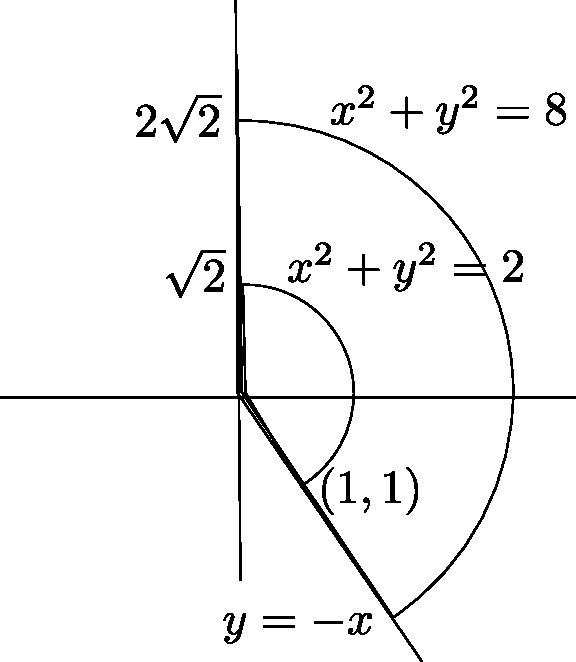
\includegraphics[width=2.2in]{T3_2b.pdf}
 \end{center}
\columnbreak
 
In polar coordinates this region is given by $-\pi/4\leq \theta\leq \pi/2$ and $\sqrt{2}\leq r\leq 2\sqrt{2}$, so we have
\begin{align*}
 A & = \int_{-\pi/4}^{\pi/2}\int_{\sqrt{2}}^{2\sqrt{2}}r\,dr\,d\theta\\
& = \frac{3\pi}{4}\left(\frac{8-2}{2}\right)\\
& = \frac{9\pi}{4}.
\end{align*}

\end{multicols}
\newpage
\item Evaluate the integral $\di \int_0^4\int_{-\sqrt{4x-x^2}}^0\sqrt{x^2+y^2}\,dy\,dx$ by converting to polar coordinates. \points{6}

\bigskip

The half-circle $y=-\sqrt{4x-x^2}$, or $x^2+y^2=4x$ (which becomes $(x-2)^2+y^2=1$ after completing the square) is given in polar coordinates by $r^2=4r\cos\theta$, or $r=4\cos\theta$. Since the region of integration is in the fourth quadrant, we have $-\pi/2\leq \theta\leq 0$, so
\begin{align*}
 \int_0^4\int_{-\sqrt{4x-x^2}}^0\sqrt{x^2+y^2}\,dy\,dx & = \int_{-\pi/2}^0\int_0^{4\cos\theta}r^2\,dr\,d\theta\\
& = \frac{64}{3}\int_{-\pi/2}^0\cos^3\theta\,d\theta\\
& = \frac{64}{3}\int_{-\pi/2}^0(1-\sin^2\theta)\cos\theta\,d\theta\\
& = \frac{64}{3}\int_{-1}^0(1-u^2)\,du\\
& = \frac{64}{3}\left(1-\frac{1}{3}\right)\\
& = \frac{128}{9}.
\end{align*}

\bigskip

\item Find the centroid (geometric center) of the triangle with vertices $(0,0)$, $(1,-3)$, and $(1,3)$. \points{8}

\bigskip

The triangle is given as a Type I region by $0\leq x\leq 1$ with $-3x\leq y\leq 3x$. The triangle has base width 6 and height 1, so its area is $A = \dfrac{1}{2}(6)(1) = 3$. Since the region is symmetric about the $x$-axis we have
\[
 \overline{y} = \frac{1}{A}\iint_D y\,dA = 0
\]
by symmetry, since $f(x,y)=y$ is an odd function of $y$. The $x$-coordinate of the centroid is given by
\begin{align*}
 \overline{x}& = \frac{1}{A}\iint_D x\,dA\\
& = \frac{1}{3}\int_0^1\int_{-3x}^{3x}x\,dx\,dy\\
& = \frac{1}{3}\int_0^1 6x^2\,dy\\
& = \frac{1}{3}(2)(1^3)\\
& = \frac{2}{3}.
\end{align*}
Thus, the centroid of the triangle is at $\left(\dfrac{2}{3},0\right)$.
\newpage

\item Set up, but do not evaluate, the integral $\di \iiint_E x^2\cos(yz)\,dV$, where $E$ is the tetrahedron with vertices $(1,0,0)$, $(0,3,0)$, and $(0,0,6)$. \points{6}

\bigskip

The tetrahedron is bounded by the coordinate planes and the plane passing through the three points other than the origin. This plane intersects the coordinate planes in the lines $3x+y=3$, $z=0$ (or $6x+2y=6$), $6x+z=6$, $y=0$, and $2y+z=6$, $x=0$. Thus, the equation of the plane must be $6x+2y+z=6$, so we can describe the region by $0\leq z\leq 6-6x-2y$ with $(x,y)$ in the triangle bounded by $x=0$, $y=0$, and $3x+y=3$, which we can write as $0\leq y\leq 3-3x$, with $0\leq x\leq 1$. Thus, we have
\[
 \iiint_E x^2\cos(yz)\,dV = \int_0^1\int_{0}^{3-3x}\int_0^{6-6x-2y}x^2\cos(yz)\,dz\,dy\,dx.
\]

\bigskip

\bigskip

\item Let $E\subseteq \R^3$ be the region bounded below by the cone $z=\sqrt{x^2+y^2}$ and above by the sphere $x^2+y^2+z^2=2z$. Express the volume of $E$ as a triple integral in {\bf both} cylindrical and spherical coordinates. You do not have to compute the volume. \points{6}

\bigskip

The sphere $x^2+y^2+z^2=2z$, or $x^2+y^2+(z-1)^2=1$, intersects the cone $z=\sqrt{x^2+y^2}$ when $z^2+z^2=2z$, which gives $z=0$ or $z=1$. The intersection at $z=0$ is where the base of the cone meets the bottom of the sphere, while the intersection at $z=1$ is the circle $z=1=x^2+y^2$. The region thus consists of the top half of the sphere, lying on top of the portion of the cone between $z=0$ and $z=1$.

In cylindrical coordinates, we have $0\leq \theta\leq 2\pi$ and $0\leq r\leq 1$, since the region projects down to the $xy$-plane onto the disk $x^2+y^2\leq 1$. The equation of the cone is simply $z=r$, while the sphere becomes $(z-1)^2 = 1-r^2$, so $z=1+\sqrt{1-r^2}$ for the top half of the sphere (positive root). Thus, the volume is given in cylindrical coordinates by
\[
 V = \int_0^{2\pi}\int_0^1\int_r^{1+\sqrt{1-r^2}}r\,dz\,dr\,d\theta.
\]
In spherical coordinates the cone is given by $\varphi = \pi/4$, so the interior of the cone corresponds to $0\leq\varphi\leq \pi/4$, and the sphere is given by $\rho^2=2\rho\cos\varphi$, or $\rho=2\cos\varphi$ (since $\rho=0$ can be obtained by setting $\varphi = \pi/2$). Since the region lies inside the sphere, we have $0\leq \rho\leq 2\cos\varphi$, and since the region is symmetric about the $z$-axis we have $0\leq \theta\leq 2\pi$. Thus, we have
\[
 V = \int_0^{2\pi}\int_0^{\pi/4}\int_0^{2\cos\varphi}\rho^2\sin\varphi\,d\rho\,d\varphi\,d\theta.
\]
\end{enumerate}

\end{document}